\section{Evaluation of BoSSS for Viscid Flows}
\frame{\tableofcontents[currentsection]}
	\subsection{Theory}
	\begin{frame}
		\frametitle{Theory -- Viscid Flow Around a Cylinder}
		\begin{columns}[t]
			\column[]{6cm}
			\vspace{-0.5cm}
			\begin{itemize}
				\item $\text{Re} \leq 40-50$: laminar steady regime
				\item $40-50 \leq \text{Re} \leq 190$: laminar vortex shedding (Kármán vortex street)
				\item $190 \leq \text{Re}$: increasing 3D effects
				\pause
				\item Characteristic values:
				\begin{itemize}
					\item Coefficient of drag $C_D$
					\item Coefficient of lift $C_L$
					\item Wake separation length $W^*$
					\item Strouhal number (frequency of vortex shedding)
				\end{itemize}
			\end{itemize}
			\column[]{6cm}
			\onslide
			\begin{figure}[ht]
				%\centering
				 \vspace{-1cm}
				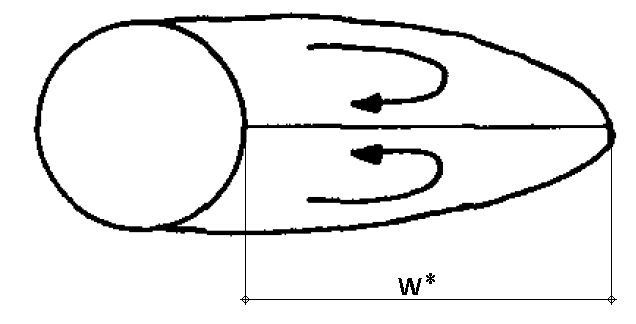
\includegraphics[width=0.6\textwidth]{img/steadyFlow_modifiedWilliamson.PNG}
				\caption{Laminar steady regime \cite{williamson} }
			\end{figure}
			\begin{figure}[htbp]
				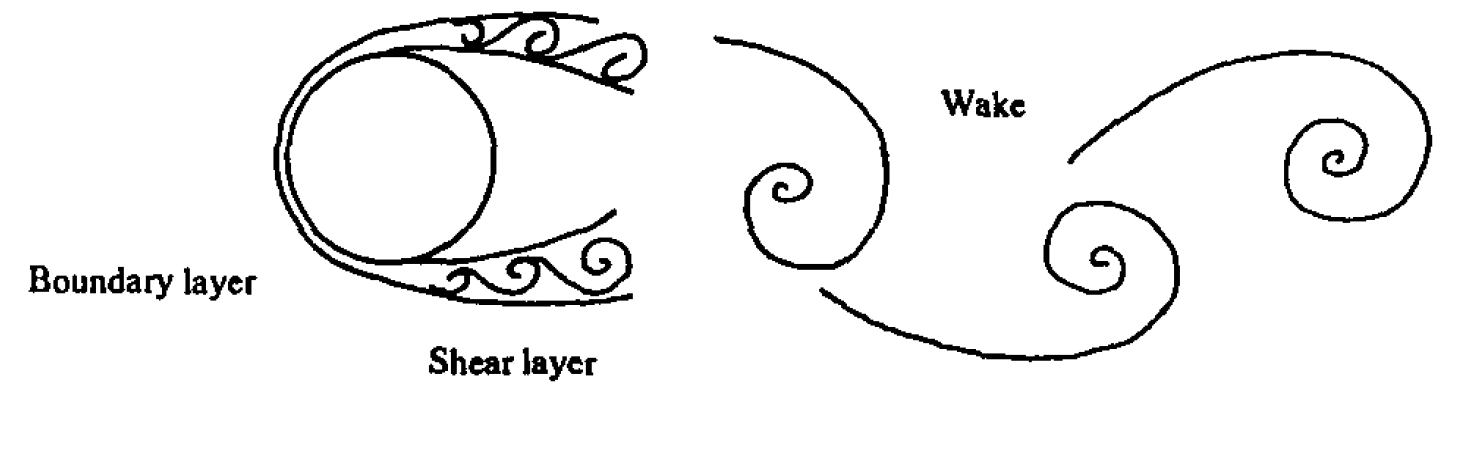
\includegraphics[width=\textwidth]{img/unsteady_Williamson.PNG}
				\caption{Kármán Vortex Street \cite{williamson} }
			\end{figure} 
		\end{columns}
	\end{frame}
%	\begin{frame}
%		\frametitle{Theory -- Laminar Steady Regime}
%		laminar steady regime
%		Bild
%		\begin{columns}[t]
%		\column[]{7cm}
%		\column[]{5cm}
%		\begin{figure}[htbp]
%			\vspace{-1cm}
%			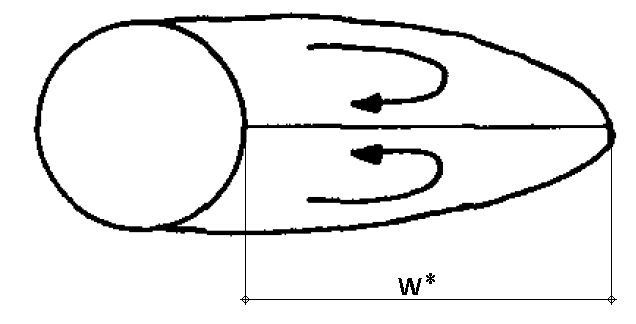
\includegraphics[width=\textwidth]{img/steadyFlow_modifiedWilliamson.PNG}
%			\caption{Recirculation Area \cite{williamson}}
%		
%		\end{figure} 
%		\end{columns}
%
%	\end{frame}	
%	\begin{frame}
%		\frametitle{Theory -- Laminar Vortex Shedding}
%		Bild
%		\begin{columns}[t]
%			\column[]{5cm}
%			\column[]{7cm}
%			\begin{figure}[htbp]
%				\vspace{-1cm}
%				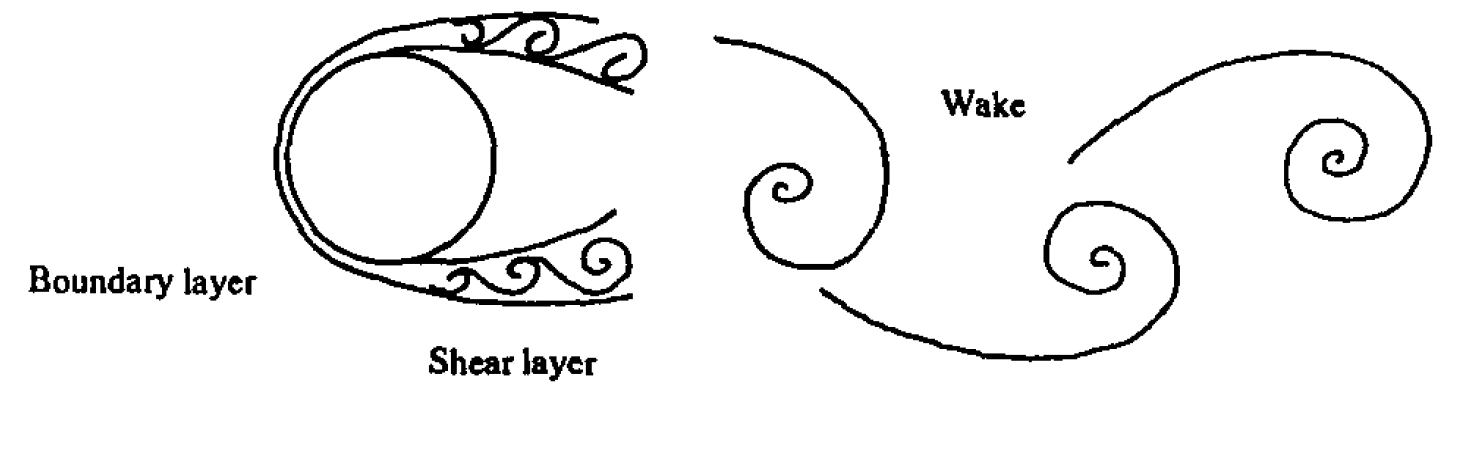
\includegraphics[width=\textwidth]{img/unsteady_Williamson.PNG}
%				\caption{Kármán Vortex Street \cite{williamson} }
%			\end{figure} 
%		\end{columns}
%		Karman vortex street
%		frequency /strouhal
%	\end{frame}	
	\subsection{Simulations}
		\begin{frame}
			\frametitle{Simulation Properties}
			\begin{columns}[t]
				\column[]{7cm}
				\vspace{-0.5cm}
			\begin{itemize}
				\item Domain:
				\begin{itemize}
					\item $-20 \leq x \leq 20$
					\item $-20 \leq y \leq 20$
					\item Cylinder with radius $r=0.5$ at $(0,0)$ \newline \MVRightarrow \, Level set $\varphi  = x^2 + y^2 -0.25$ set as  \color{myred} isothermal wall \color{black}
				\end{itemize}
				\pause
				\item Variation of mesh size: 40, 60 and 80 cells per direction
				\pause
				\item Variation of polynomial degree $1 \leq P \leq 3$
				\pause
				\item Constant agglomeration threshold $\alpha = 0.3$ \\[10pt]
				\onslide
				\bluedot Supersonic inlet
				\reddot Isothermal wall
			\end{itemize}
			\column[]{5.5cm}
			\onslide
			\vspace{-0.8cm}
			\begin{figure}[htbp]
				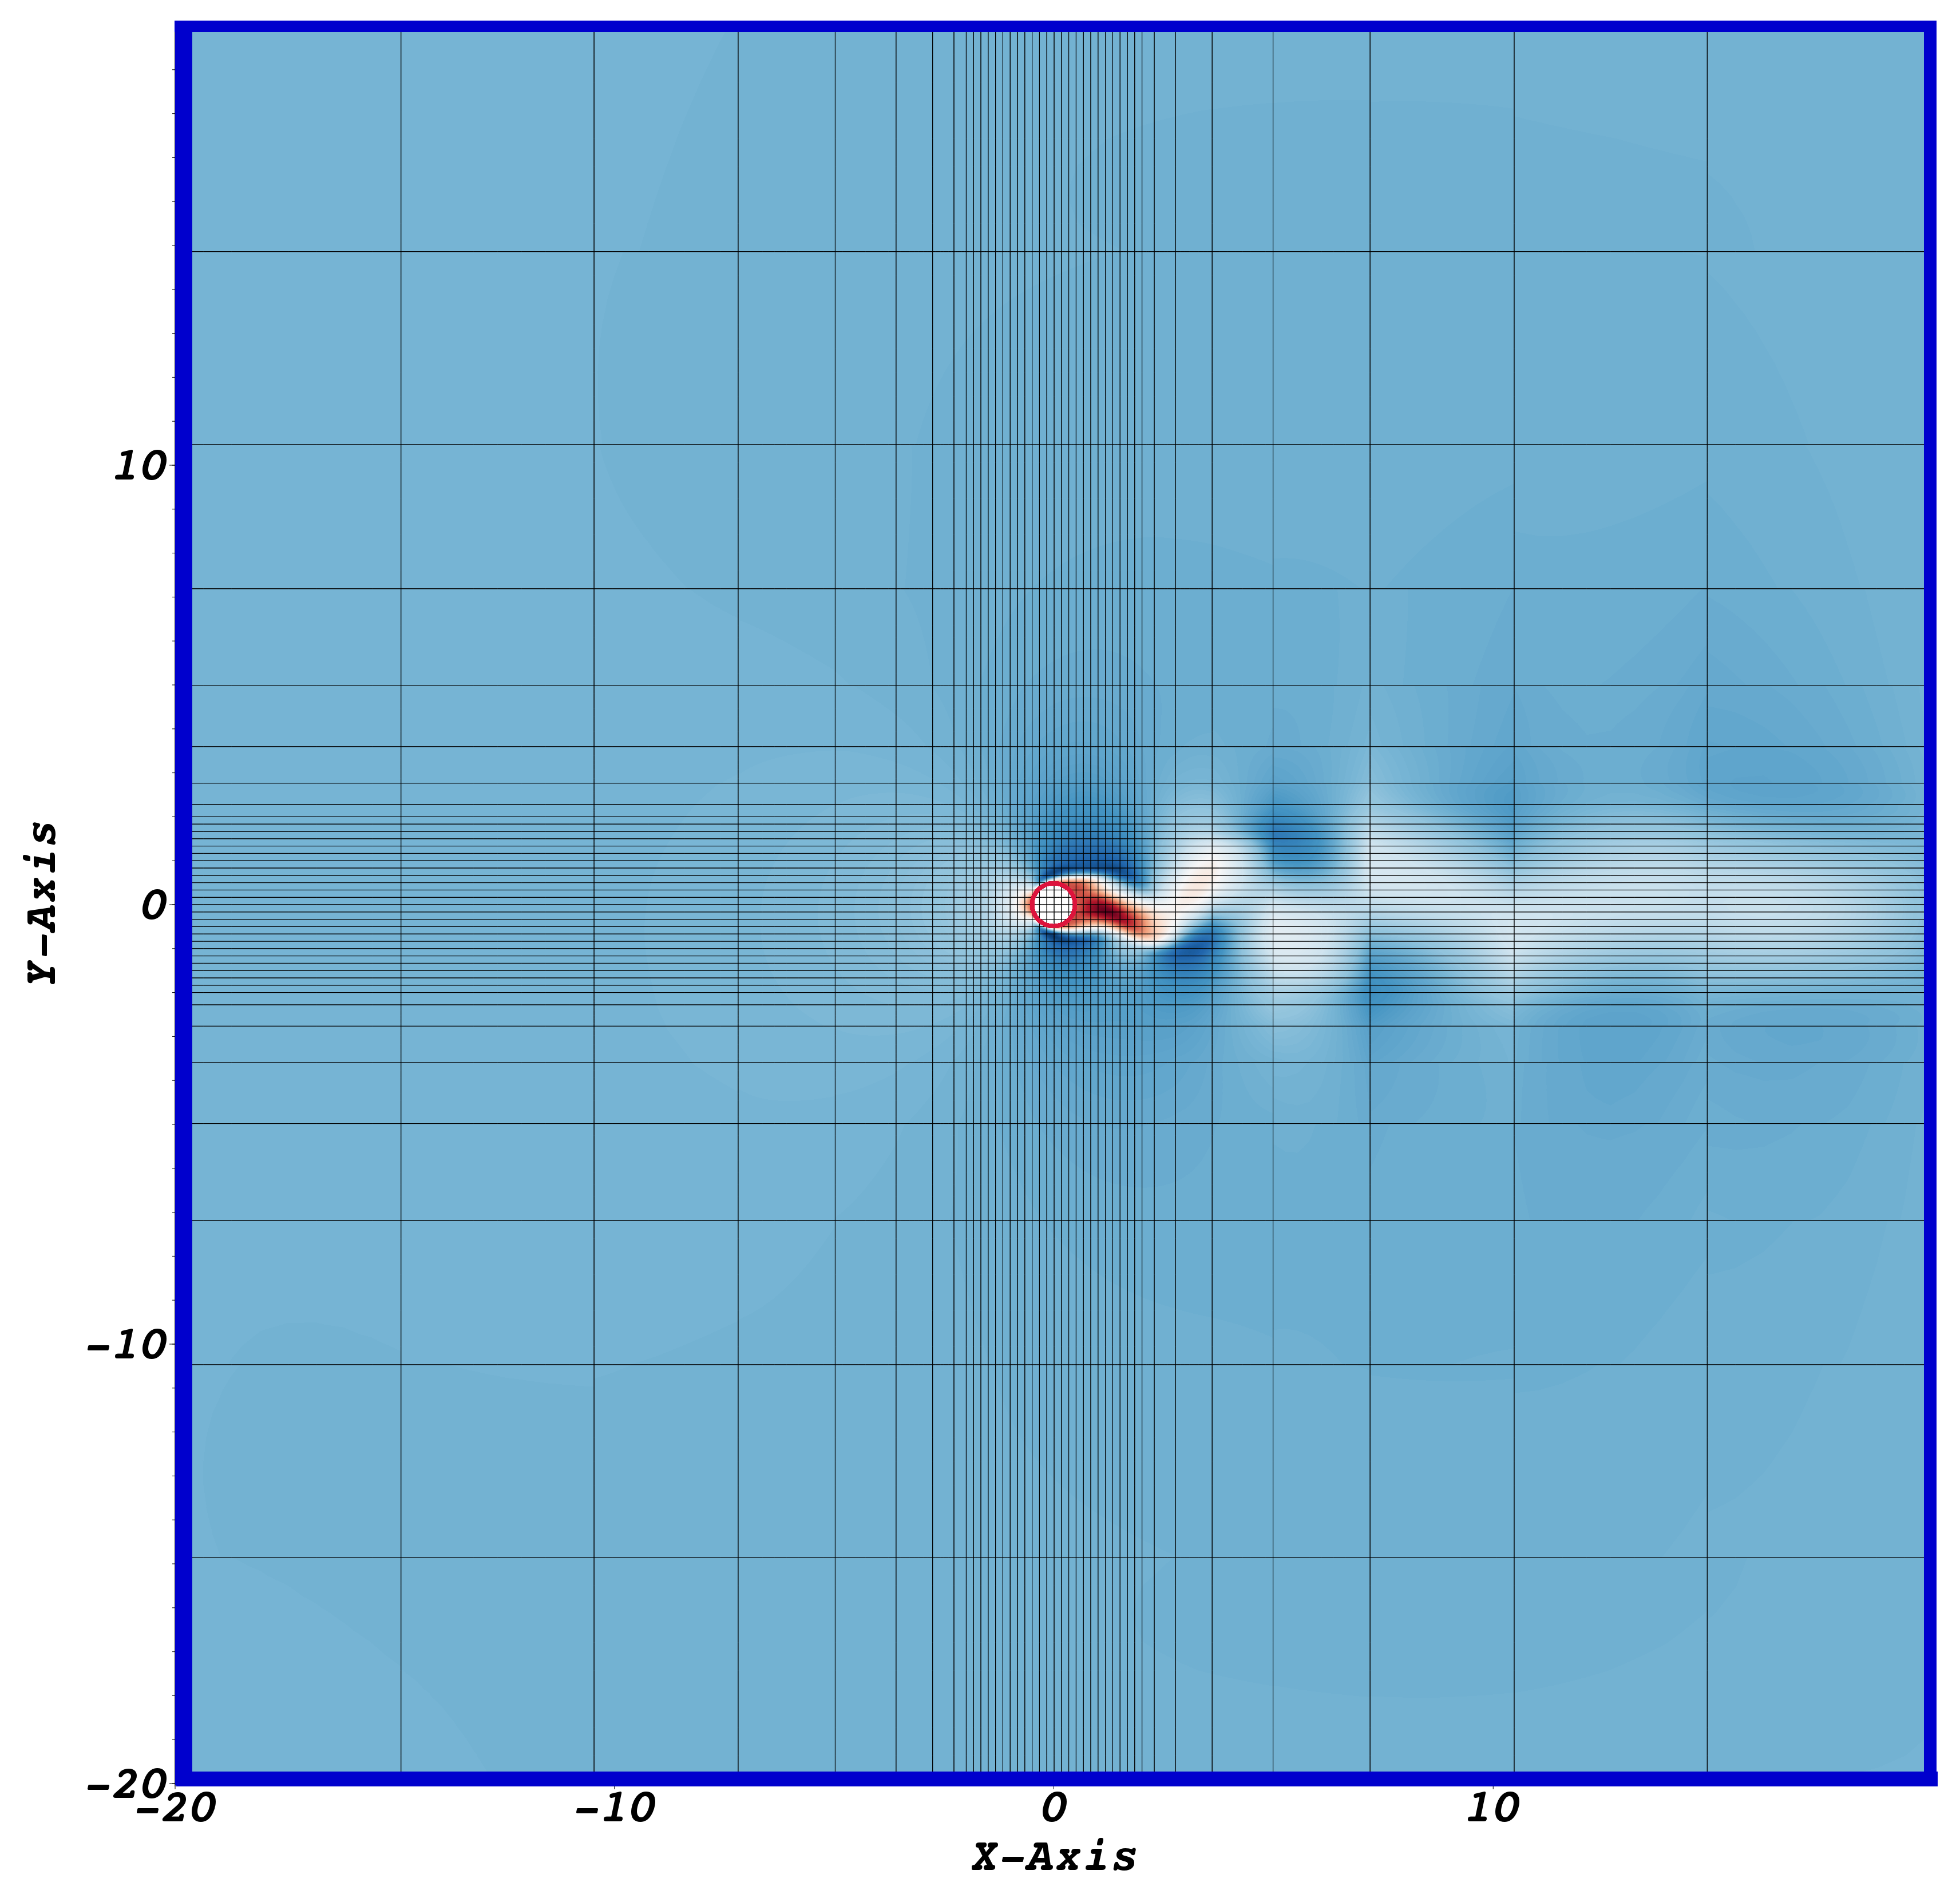
\includegraphics[width=\textwidth]{img/mesh40.PNG}
				\caption{Coarsest mesh with $40 \times 40$ cells}
			\end{figure} 
%			\begin{itemize}
%				\bluedot Supersonic inlet
%				\reddot Isothermal wall
%			\end{itemize}
		\end{columns}
%			simulation parameter
%			gitter
%			cD, CL, W*, St
		\end{frame}
		\begin{frame}
			\frametitle{Compared Values}
				\begin{columns}
					\column[]{8cm}
			
			\begin{itemize}			
				\item Steady flow simulations for $\text{Re = 20}$ and $\text{Re = 40}$:
				\begin{itemize}
					\item Coefficient of drag $C_D$
					\item Wake separation length $W^*$ \newline \MVRightArrow \, found from evaluating $x$ at $y=0$ where $x$-velocity $u=0$
				\end{itemize}
				\pause
				\item Unsteady flow simulations for $\text{Re = 100}$ and $\text{Re = 200}$:
				\begin{itemize}
					\item Coefficient of drag $C_D$
					\item Coefficient of lift $C_L$
					\item $\text{St}$ found from evaluating frequency of $C_L$
				\end{itemize}	
			\end{itemize}	
			\column[]{4cm}
			\onslide
			\begin{flalign*}
				C_D &= \tfrac{d}{q_\infty L_\infty}\\
				C_L &= \tfrac{l}{q_\infty L_\infty}\\
				\text{St} &= \dfrac{f L_\infty}{V_\infty}\\
				d&: 	\text{drag force}\\
				l&:	\text{lift force}\\
				q_\infty&:	\text{dynamic pressure}\\
				L_\infty&: \text{cylinder diameter}\\
				V_\infty&: \text{flow velocity}\\
			\end{flalign*}
			\end{columns}
		\end{frame}
		\begin{frame}[allowframebreaks]
			\frametitle{Simulation at $\text{Re = 20}$}
			\begin{table}[htp]
				\small
				\centering
				\begin{tabular}{|l|l|c|c|c|}
					\hline
					\rule{0pt}{2,3ex}$\text{Re}=20$                              & Source                             & 2D/3D & $W^*$ & $C_D$ \\ \hline
					\rule{0pt}{2,3ex}\multirow{3}{*}{\begin{minipage}{2.8cm}Numerical --\newline Incompressible\end{minipage}} & Dennis and Chang           & 2D    & $0.94$     & $2.05$     \\ \cline{2-5} 
					\rule{0pt}{2,3ex}& Fornberg                 & 2D    & $0.91$     & $2.00$     \\ \cline{2-5} 
					\rule{0pt}{2,3ex}& Linnick and Fasel         & 2D    &$ 0.93 $    & $2.06$     \\ \hline
					\rule{0pt}{2,3ex}\multirow{2}{*}{Experimental}               & Coutanceau and Bouard       & -     & 0.93    & -     \\ \cline{2-5} 
					\rule{0pt}{2,3ex}& Tritton             & -     & -     & $2.09$     \\ \hline
					\rule{0pt}{2,3ex}\multirow{3}{*}{\begin{minipage}{2.8cm}Numerical --\newline Compressible\end{minipage}}     & Brehm, Hader and Fasel (Ma = 0.1) & 3D    & $0.96$     &$ 2.02$     \\ \cline{2-5} 
					\rule{0pt}{2,3ex}& Ayers                 & 2D    & $0.975$     & $2.06 $    \\ \cline{2-5} 
					\rule{0pt}{2,3ex}& \textbf{Present Results:}                   & \textbf{2D}    & $\mathbf{0.928}$     & $\mathbf{2.136}$     \\ \hline
				\end{tabular}	
			\end{table}
			\begin{itemize}
				\item $W^*$ coincides with literature, $C_D$ much too high
			\end{itemize}
		%	re 20 tabelle, plot, drag over time, vorticity
%		\end{frame}
%		\begin{frame}
\vspace{4cm}
			\begin{columns}[t]
				\column[]{5cm}
				\begin{itemize}
					\item None of the values lies in the range found in literature
					\item Simulation for $P=2$, $\text{CpD}=80$ should be examined again
					\item Overall, $P=1$ behaviour as expected,  $P=2$ and $3$ yield much too high results
				\end{itemize}
				\column[]{7cm}
				\begin{figure}[htp]
					\centering		
					\includestandalone[width=\textwidth]{re20cdwerte}
				\end{figure}
			\end{columns}
		\end{frame}
		\begin{frame}[allowframebreaks]
			\frametitle{Simulation at $\text{Re = 40}$}
			\begin{table}[htp]
				\small
				\centering
				\begin{tabular}{|l|l|c|c|c|}
					\hline
					\rule{0pt}{2,3ex}$\text{Re}=40$                              & Source                             & 2D/3D & $W^*$ & $C_D$ \\ \hline
					\rule{0pt}{2,3ex}\multirow{3}{*}{\begin{minipage}{2.8cm}Numerical --\newline Incompressible\end{minipage}} & Dennis and Chang          & 2D    & $2.35$     & $1.52 $    \\ \cline{2-5} 
					\rule{0pt}{2,3ex}& Fornberg                & 2D    & $2.24$     & $1.50 $   \\ \cline{2-5} 
					\rule{0pt}{2,3ex}& Linnick and Fasel         & 2D    &$ 2.28$     & $1.54  $   \\ \hline
					\rule{0pt}{2,3ex}\multirow{2}{*}{Experimental}               & Coutanceau and Bouard      & -     & $2.13 $  & -     \\ \cline{2-5} 
					\rule{0pt}{2,3ex}& Tritton                & -     & -     & $1.59 $    \\ \hline
					\rule{0pt}{2,3ex}\multirow{3}{*}{\begin{minipage}{2.8cm}Numerical --\newline Compressible\end{minipage}}     & Brehm, Hader and Fasel (Ma = 0.1) & 3D    & $2.26$     & $1.51 $    \\ \cline{2-5} 
					\rule{0pt}{2,3ex}& Ayers                 & 2D    & $2.250 $    & $1.605$     \\ \cline{2-5} 
					\rule{0pt}{2,3ex}& \textbf{Present Results:}                   & \textbf{2D}    & $\mathbf{2.201}$     & $\mathbf{1.608} $    \\ \hline
				\end{tabular}	
			\end{table}
			\begin{itemize}
				\item $W^*$ coincides with literature, $C_D$ slightly high
			\end{itemize}
%			re 40 tabelle, plot, drag over time, vorticity 
%		\end{frame}
%		\begin{frame}
\vspace{1cm}
			\begin{columns}[t]
				\column[]{5cm}
				\begin{itemize}
					\item Better results than for $\text{Re=20}$
					\item Simulation for $P=2$, $\text{CpD}=80$ once again yields discordant values
					\item $P=2$ and $P=3$ quite high compared to literature
				\end{itemize}
				\column[]{7cm}
				\begin{figure}[htp]
					\centering		
					\includestandalone[width=\textwidth]{re40cdwerte}
				\end{figure}
			\end{columns}
		\end{frame}
		\begin{frame}
			\frametitle{Comparison of $\text{Re = 20}$ and $\text{Re = 40}$}
			\begin{center}
		\vspace{-0.3cm}
			\scalebox{0.8}{
				\begin{minipage}{\the\textwidth}
			\begin{table}[htp]
				\begin{tabular}{|c|c|c|}
					\hline
					& $W^*$   & $C_D$   \\ \hline
					$\text{Re}=20$ & $0.928$ & $2.136$ \\ \hline
					$\text{Re}=40$ & $2.201$ & $1.608$ \\ \hline
				\end{tabular}
			\end{table}
		\end{minipage}
		}
	\end{center}
			\begin{figure}
				\vspace{-0.5cm}
				\centering
				\subfloat[$\text{Re = 20}$]{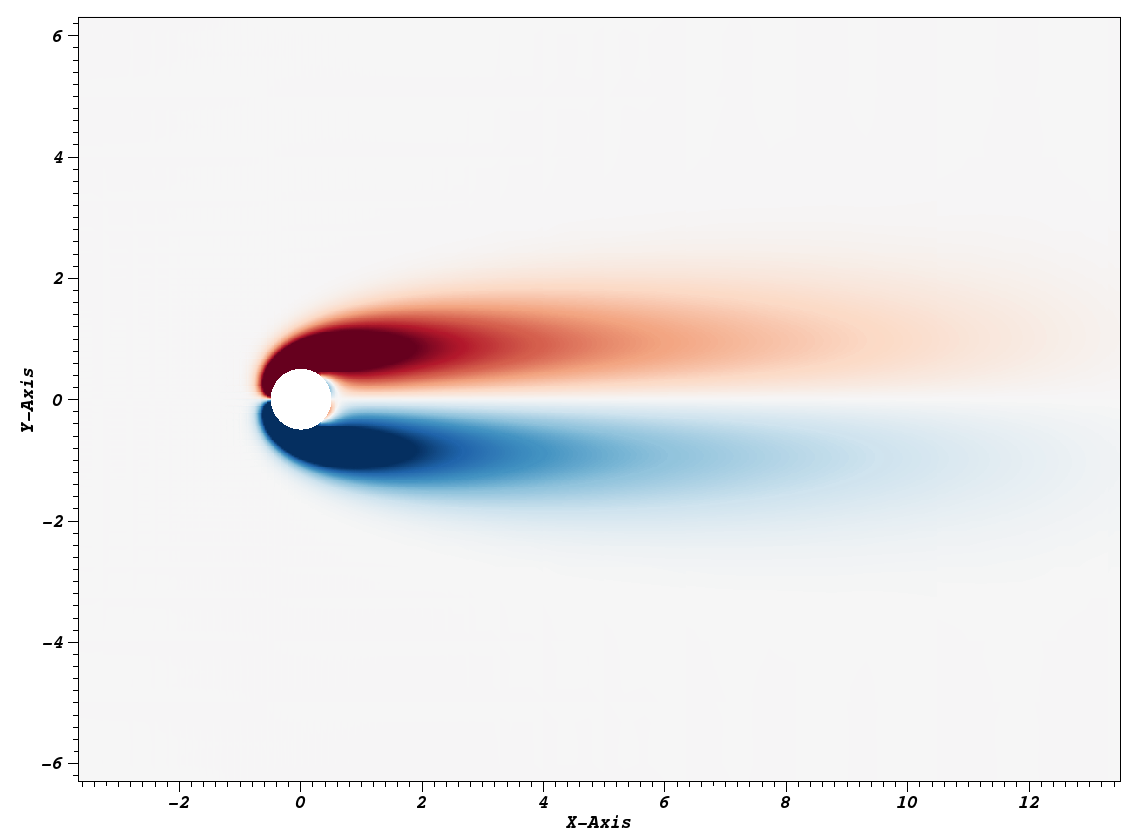
\includegraphics[width=0.45\textwidth]{img/Re20DG3CpD60.png}}
				\subfloat[$\text{Re = 40}$]{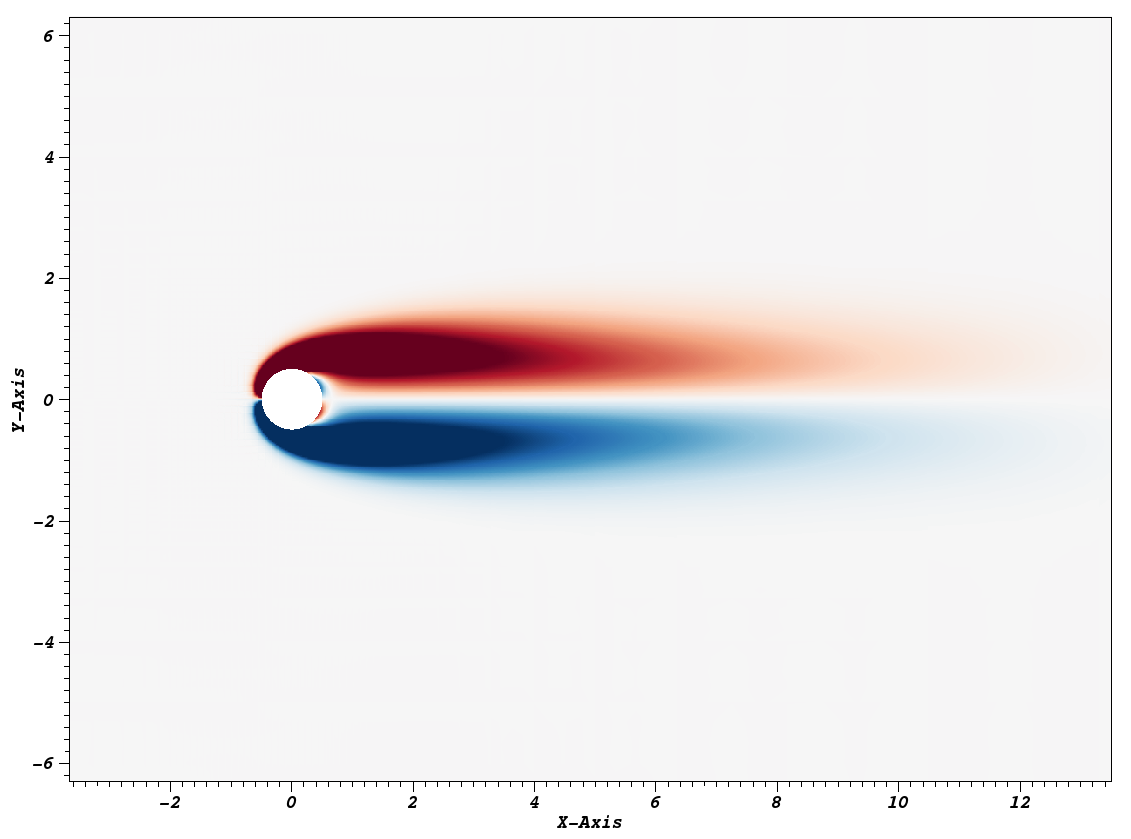
\includegraphics[width=0.45\textwidth]{img/Re40DG3CpD60.png}}
			\end{figure}
	\end{frame}
		\begin{frame}[allowframebreaks]
			\frametitle{Simulation at $\text{Re = 100}$}
			\vspace{-0.3cm}
			\scalebox{0.7}{
					\begin{minipage}{\the\textwidth}
			\begin{table}[htp]
				\centering
				\begin{tabular}{|l|l|c|c|c|c|}
					\hline
					\rule{0pt}{2,3ex}$\text{Re}=100$                              & Source                             & 2D/3D & $St$ & $C_D$ & $C_L$\\ \hline
					\rule{0pt}{2,3ex}\multirow{7}{*}{\begin{minipage}{2.8cm}Numerical --\newline Incompressible\end{minipage}} & Gresho, Chan, Lee, et al.           & 2D    & $0.18$     & $1.76$ & -   \\ \cline{2-6} 
					\rule{0pt}{2,3ex}& Linnick and Fasel ($\lambda = 0.056$)                 & 2D    & $0.169$     & $1.38 \pm 0.010$  &  $\pm  0.337 $\\ \cline{2-6} 
					\rule{0pt}{2,3ex}& Linnick ad Fasel ($\lambda = 0.023$)                  & 2D    & $0.1696 $   & $1.34 \pm 0.009$  & $ \pm 0.333 $\\ \cline{2-6} 
					\rule{0pt}{2,3ex}& Persillon and Braza                  & 2D    & $0.165  $   &$ 1.253 $ & -  \\ \cline{2-6} 
					\rule{0pt}{2,3ex}& Saiki and Biringen                 & 2D    &$ 0.171  $   & $1.26 $ &  - \\ \cline{2-6} 
					\rule{0pt}{2,3ex}& Persillon and Braza                   & 3D    & $0.164$     & $1.240 $ & -  \\ \cline{2-6} 
					\rule{0pt}{2,3ex}& Liu, Zheng and Sung         & 3D    &$ 0.165 $    & $1.35 \pm 0.012$  &$ \pm 0.339 $ \\ \hline
					\rule{0pt}{2,3ex}\multirow{2}{*}{Experimental}               & Berger and Wille     & -     &$ 0.16-0.17 $   & -    & -\\ \cline{2-6} 
					\rule{0pt}{2,3ex}& Clift, Grace and Weber               & -    & -     &$ 1.24 $ &  - \\ \cline{2-6} 
					\rule{0pt}{2,3ex}& Williamson              & -     &$ 0.164  $  & -   & - \\ \hline
					\rule{0pt}{2,3ex}\multirow{3}{*}{\begin{minipage}{2.8cm}Numerical -- \newline Compressible\end{minipage}}     & Brehm, Hader and Fasel (Ma = 0.1) & 3D    & $0.165$    &$ 1.32 \pm 0.01  $  & $\pm 0.32 $\\ \cline{2-6} 
					\rule{0pt}{2,3ex}& Ayers                  & 2D    &$ 0.167$     & $1.371 \pm 0.011 $ &$ \pm 0.333 $\\ \cline{2-6} 
					\rule{0pt}{2,3ex}& \textbf{Present Results:}                   & \textbf{2D}    & $\mathbf{0.1669}$     & $\mathbf{1.3593 \pm 0.00805}$  &  $\mathbf{\pm 0.3291}$ \\ \hline
				\end{tabular}	
			\end{table}
				\end{minipage}
			}
			\vspace{-0.1cm}
			\begin{itemize}
				\item All values coincide with literature
			\end{itemize}
%			
			\begin{columns}[t]
				\column[]{5cm}
				\begin{itemize}
					\item Higher degree values lie in expected range
					\item Values which should be most accurate ($P=2$, $\text{CpD}=80$ and $P=3$, $\text{CpD}=60$) produce rather high results
					\item $P=2$ seems to converge against $P=3$, $\text{CpD}=60$ value
				\end{itemize}
				\column[]{7cm}
				\begin{figure}[htp]
					\centering		
					\includestandalone[width=\textwidth]{re100cdwerte}
				\end{figure}
			\end{columns}
			
		\end{frame}
		\begin{frame}[allowframebreaks]
			\frametitle{Simulation at $\text{Re = 200}$}
			\scalebox{0.7}{
				\begin{minipage}{\the\textwidth}
			\begin{table}[htp]
				\centering
				\begin{tabular}{|l|l|c|c|c|c|}
					\hline
					\rule{0pt}{2,3ex}$\text{Re}=200$                              & Source                             & 2D/3D & $St$ & $C_D$ & $C_L$\\ \hline
					\rule{0pt}{2,3ex}\multirow{9}{*}{\begin{minipage}{2.8cm}Numerical --\newline Incompressible\end{minipage}} & Belov, Martinelli and Jameson           & 2D    & $0.193$     & $1.19 \pm 0.042$ & $\pm 0.64$   \\ \cline{2-6} 
					\rule{0pt}{2,3ex} & Gresho, Chan, Lee et al.             & 2D    & $0.21$     & $1.76$ & -   \\ \cline{2-6} 
					\rule{0pt}{2,3ex}& Linnick and Fasel ($\lambda = 0.056$)                 & 2D    & $0.199$     & $1.37 \pm 0.046$  &  $\pm  0.70$\\ \cline{2-6} 
					\rule{0pt}{2,3ex}& Linnick and Fasel ($\lambda = 0.023$)                  & 2D    & $0.197 $   & $1.34 \pm 0.044$  & $ \pm 0.69$\\ \cline{2-6} 
					\rule{0pt}{2,3ex}& Miyake, Sakamoto, Tokunaga et al.               & 2D    & $0.196$   &$1.34 \pm 0.043 $ & $\pm 0.67$  \\ \cline{2-6} 
					\rule{0pt}{2,3ex}&  Persillon and Braza               & 2D    & $0.198  $   &$ 1.321 $ & -  \\ \cline{2-6} 
					\rule{0pt}{2,3ex}& Saiki and Biringen                 & 2D    &$ 0.197  $   & $1.18 $ &  - \\ \cline{2-6} 
					\rule{0pt}{2,3ex}& Persillon and Braza                 & 3D    & $0.181$     & $1.306 $ & -  \\ \cline{2-6} 
					\rule{0pt}{2,3ex}& Liu, Zheng and Sung           & 3D    &$ 0.192 $    & $1.31 \pm 0.049$  &$ \pm 0.69 $ \\ \hline
					\rule{0pt}{2,3ex}\multirow{2}{*}{Experimental}               & Berger and Wille      & -     &$ 0.18-0.19 $   & -    & -\\ \cline{2-6} 
					\rule{0pt}{2,3ex}& Clift, Grace and Weber                 & -    & -     &$ 1.16 $ &  - \\ \cline{2-6} 
					\rule{0pt}{2,3ex}& Williamson               & -     &$ 0.181  $  & -   & - \\ \hline
					\rule{0pt}{2,3ex}\multirow{3}{*}{\begin{minipage}{2.8cm}Numerical --\newline Compressible\end{minipage} }    &  Brehm, Hader and Fasel (Ma = 0.1) & 3D    & $0.192$    &$ 1.3 \pm 0.04  $  & $\pm 0.66 $\\ \cline{2-6} 
					\rule{0pt}{2,3ex}& Ayers                  & 2D    &$ 0.201$     & $1.371 \pm 0.011 $ &$ \pm 0.70 $\\ \cline{2-6} 
					\rule{0pt}{2,3ex}& \textbf{Present Results:}                   & \textbf{2D}    & $\mathbf{0.2002}$     & $\mathbf{1.344 \pm 0.0462}$  &   $\mathbf{\pm 0.6887}$\\ \hline
				\end{tabular}	
			\end{table}
		\end{minipage}
		}
			\begin{columns}[t]
				\column[]{5cm}
				\begin{itemize}
					\item All values seen in table coincide with literature
					\item Compared to 3D results by \cite[Brehm et al.]{brehm} all values slightly higher
					\item All $C_D$ values (except for the least accurate one) lie in expected range
					\item $P=2$ seems to converge against higher value than $P=1$
				\end{itemize}
				\column[]{7cm}
				\begin{figure}[htp]
					\centering		
					\includestandalone[width=\textwidth]{re200cdwerte}
				\end{figure}
			\end{columns}
		\end{frame}
		\begin{frame}[allowframebreaks]
			\frametitle{Comparison of $\text{Re = 100}$ and $\text{Re = 200}$}
			\begin{columns}[t]
				\column[]{6.5cm}
				\vspace{-1cm}
				\begin{figure}[htp]
					\centering		
					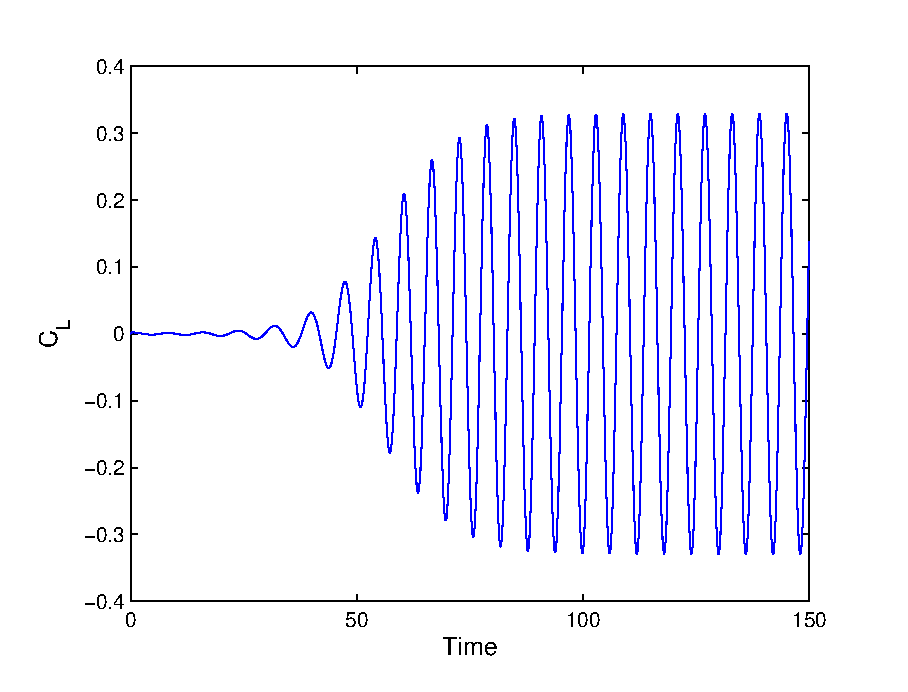
\includegraphics[width=\textwidth]{img/re100dg3cpd60cl.eps}
				\end{figure}
%				\vspace{-0.5cm}

				\column[]{6.5cm}
				\vspace{-1cm}
			\begin{figure}[htp]
				\centering		
				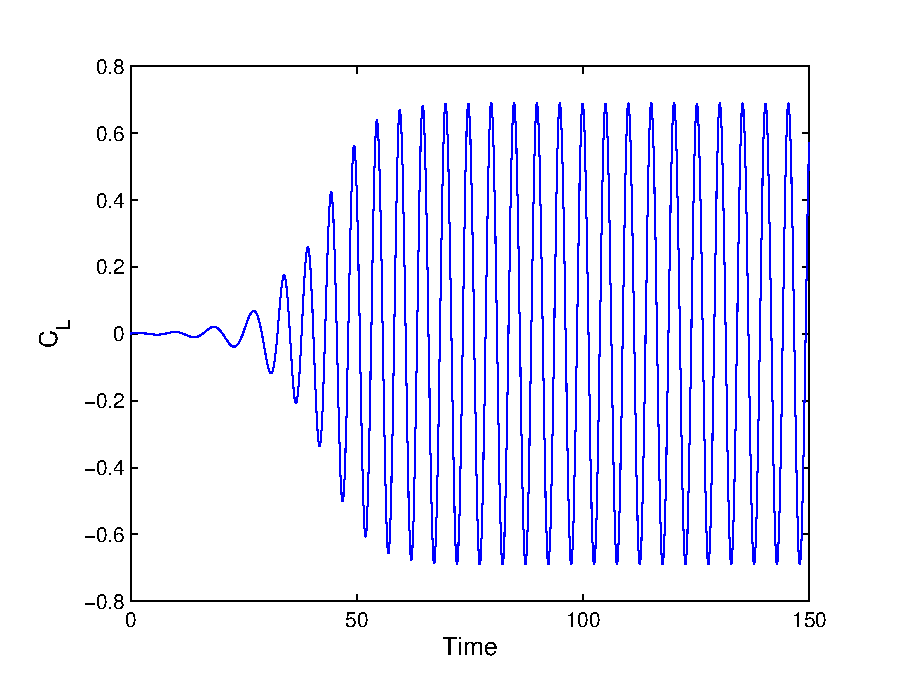
\includegraphics[width=\textwidth]{img/re200dg3cpd60cl.eps}
			\end{figure}
			\end{columns}
			\begin{itemize}
				\item Higher amplitude and frequency for $C_L$ at $\text{Re}=200$ compared to $\text{Re}=100$
				\item Steady state is reached earlier
			\end{itemize}
			\vspace{5cm}
			\begin{columns}[t]
				\column[]{6cm}
				\vspace{-1cm}
				\begin{figure}[htp]
					\centering		
					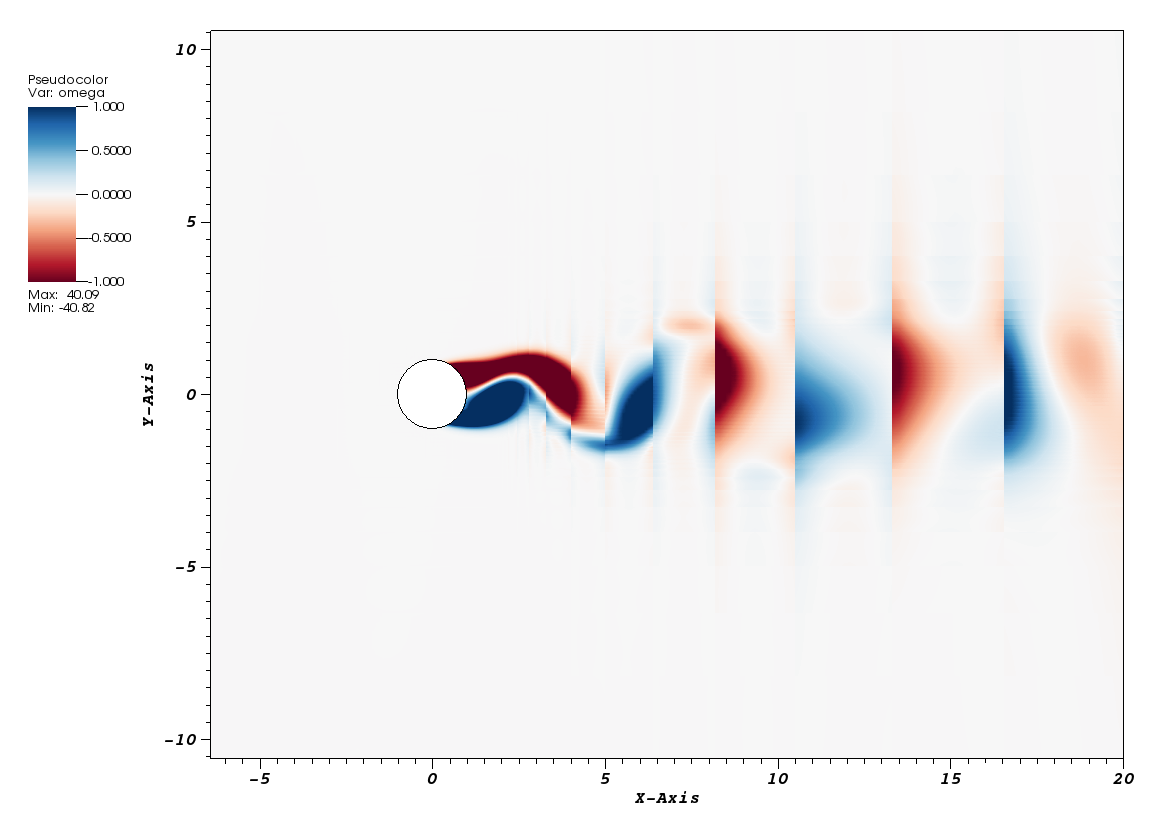
\includegraphics[width=\textwidth]{img/re100dg3cpd60.png}
				\end{figure}
				\column[]{6cm}
				\vspace{-1cm}
				\begin{figure}[htp]
					\centering		
					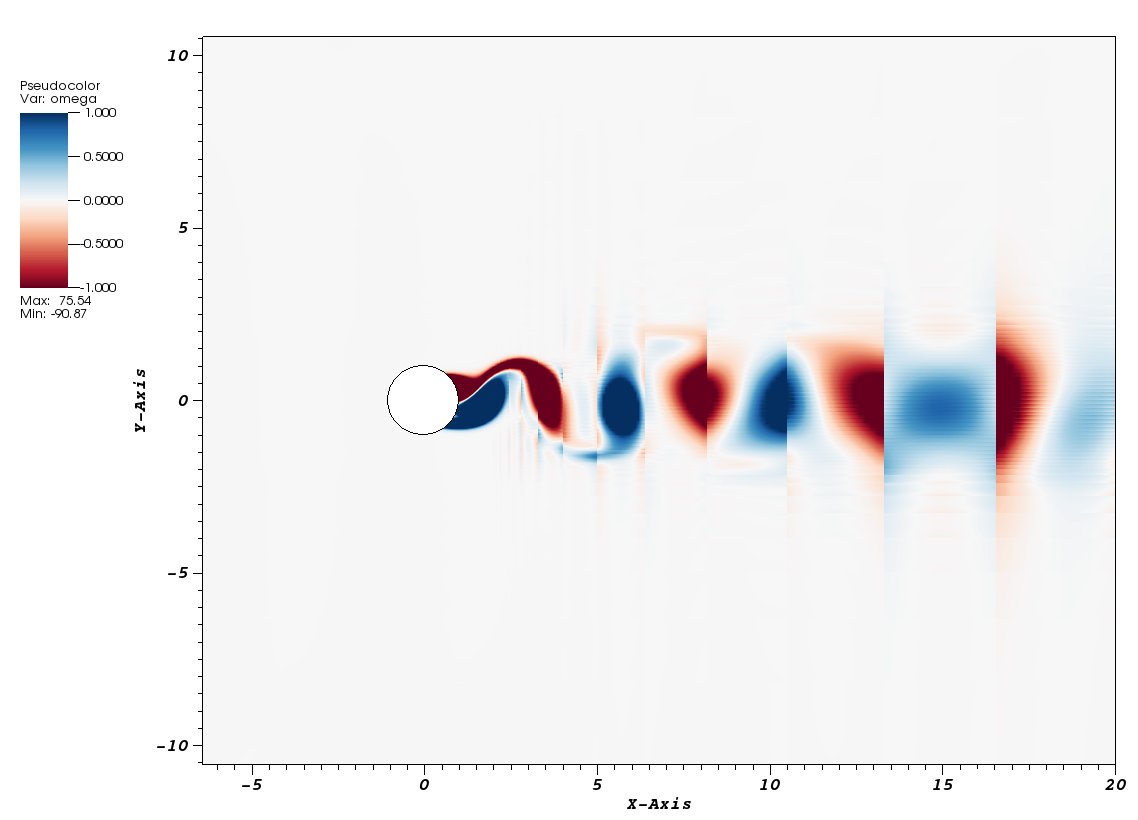
\includegraphics[width=\textwidth]{img/re200dg3cpd60.png}
				\end{figure}
			\end{columns}
			\begin{center}
			\scalebox{0.8}{
				\begin{minipage}{\the\textwidth}
					\begin{table}[htp]
						\begin{tabular}{|c|c|c|c|}
							\hline
							& $St$   & $C_D$  & $C_L$ \\ \hline
							$\text{Re}=100$ & $0.1669$ & $1.359\pm 0.00805$ & $\pm 0.3291$ \\ \hline
							$\text{Re}=200$ & $0.2002$ & $1.344 \pm 0.0462$ & $\pm 0.6887$ \\ \hline
						\end{tabular}
					\end{table}
				\end{minipage}
			}
		\end{center}
		\end{frame}